\documentclass{article}
\usepackage[utf8]{inputenc}
\usepackage[T1]{fontenc}
\usepackage{lmodern}
\usepackage[english]{babel}
\usepackage{amsmath, amssymb, amsthm, stmaryrd}
\usepackage{tikz}
\usetikzlibrary{calc, decorations.text}

\newcommand{\G}{\mathbb{G}}
\newcommand{\D}{\mathbb{D}}

\newtheorem{theorem}{Theorem}
\newtheorem{lemma}{Lemma}
\newtheorem{definition}{Definition}

\title{Extending results for an arbitrary set of generations}
\author{}

\begin{document}

\maketitle

\section{Notations}

We denote by $\G$ the set of generations, and $Y$ the set of utility values.\\
The set of utility streams is $X=Y^\G$.\\
$\kappa$ is a non-empty family of subsets of $\G$, stable by union and which doesn't
contain $\emptyset$.\\
$\mu$ is a subgroup of $\mathfrak{S}_\G$.

\section{Axioms}

We define the $\kappa$-relation as:
\[<_\kappa = \{(x,y)\in X^2|\forall i\in \G, x_i \leq y_i \land
\{j \in \G | x_j < y_j\}\in\kappa\}\]
$<_\kappa$ is a strict order:
\begin{itemize}
  \item Irreflexive since $\emptyset\not\in\kappa$.
  \item Asymmetric because $x<_\kappa y$ implies that for all $i\in\G$,
        $x_i\leq y_i$, and there exists $j$ such that $x_j < y_j$. Hence
        it is not possible to have $x<_\kappa y$ and $y<_\kappa x$.
  \item Transitive since $\kappa$ is stable by union.
\end{itemize}
We note $\leq_\kappa$ the reflexive closure of $<_\kappa$.\smallskip\par

\begin{definition}{Social Welfare Function (SWF)}
  A social welfare function is a function from a set of utility streams
  to a totally ordered set.
\end{definition}

\textbf{$\kappa$-Pareto}:
\[\forall x,y\in X, x <_\kappa y \Rightarrow x \prec y\]

\textbf{$\mu$-anonymity}:
\[\forall\sigma\in\mu,\forall x\in X, x \sim \sigma x\]

These two axioms can be extended as usual over social welfare functions.

\section{Grading principle}
\ \par
\textbf{$\kappa$-$\mu$ grading principle}:
\[\precsim_{\kappa\mu} = \{(x,y)\in X^2 |
\exists\sigma\in\mu, x \leq_\kappa \sigma y\}\]

Adaptation of theorem 1 in \cite{svensson80}:
\begin{theorem}
    $\precsim_{\kappa\mu}$ is a $\mu$-anonymous quasi-ordering on $X$, and
    $\kappa$-paretian if...
\end{theorem}
\begin{proof}
    \textbf{Reflexivity}: we can take $\sigma = Id\in\mu$ since $\mu$ is a
    subgroup of $\mathfrak{S}_\G$.\\
    \textbf{Transitivity}: if $x,y,z\in X$ such that $x \precsim_{\kappa\mu} y$ and
    $y \precsim_{\kappa\mu} z$,
    we take $\sigma,\sigma'\in \mu$ such that $x\leq_\kappa \sigma y$ and
    $y\leq_\kappa \sigma' z$. We have $x\leq_\kappa (\sigma\circ\sigma')z$,
    and $\sigma\circ\sigma'\in\mu$ since $\sigma$ and $\sigma'$ are both in $\mu$.\\
    \textbf{$\mu$-anonymity}: if $x\in X$ and $\sigma\in\mu$, then
    $x\leq_\kappa\sigma^{-1}\sigma x$ with $\sigma^{-1}\in\mu$,
    therefore $x \precsim_{\kappa,\mu} \sigma x$. On the other hand,
    $\sigma x \leq_{\kappa}\sigma x$, hence $x \sim_{\kappa, \mu}\sigma x$.\\
    \textbf{$\kappa$-Pareto}: if we have $x,y\in X$ with $x<_\kappa y$, is there a
    $\sigma\in \mu\mathfrak{S}_\G$ such that $y\leq_\kappa \sigma x$?
\end{proof}

\section{Existence of SWF}

\begin{theorem}
  Suppose $\kappa$ contains only finite subsets of $\G$, and $\mu$ contains only permutation
  with finite support. Suppose $X=\mathbb Q^{\mathbb N}$.

  Then there exists a SWF $W:X\to\mathbb R$ which is $\kappa$-Pareto and $\mu$-anonymous.
\end{theorem}

\begin{proof}
  Define the relation $\preceq$ on $X$ by $a\preceq b$ iff exists $n\in\mathbb N^*$, $c_1,...,c_n\in X$ and
  $\sigma_1,...,\sigma_{2n-2}\in\mu$ such that $a=c_1$, $b=c_n$ and $\forall 1\leq i\leq n-1, \sigma_{2i-1}(c_i)<_\kappa\sigma_{2i}(c_{i+1})$.

  $\preceq$ is a reflexive by taking $n=1$ and transitive thanks to its chain form,
  so it is a preorder. \medskip

  Define the relation $\sim$ on $X$ by $a\sim b$ iff exists $n\in\mathbb N^*$ and $c_1,...,c_n\in X$
  such that $a=c_1$, $b=c_n$ and $\forall 1\leq i\leq n-1, c_i\preceq c_{i+1}$ or $c_{i+1}\preceq c_i$.

  $\sim$ is somehow the smallest equivalence relation containing $\preceq$.

  Denote by $\tilde{a}$ the equivalence class of $a$. \medskip

  Let $a\in X$. Let $A_n$ be the set of elements that are related to $a$ at distance
  $n$, i.e. $A_n=\{b\,|\, \exists c_1,...,c_n\in X, \sigma_1,...,\sigma_{2n-2}\in\mu, a=c_1 \wedge b=c_n \wedge \forall 1\leq i\leq n-1, \left(\sigma_{2i-1}(c_i)<_\kappa\sigma_{2i}(c_{i+1}) \vee \sigma_{2i}(c_{i+1})<_\kappa\sigma_{2i-1}(c_i)\right)\}$.
\end{proof}


\medskip
Adaptation of theorem 1 of \cite{basumitra03}:
\begin{theorem}
  Suppose $\kappa$ contains a subset $k$ of $\G$ such that $\mathbb G\setminus k$ is infinite,
  $|\mathbb G\setminus k|\geq |k|$ and $\mu$ contains the permutations of size $2|k|$.

  Let $\mathbb S$ be an totally ordered set such as there exists a subset $\D$ dense in
  $\mathbb S$ such that $|\D|\leq |\G\setminus k|$ and $|\D|<|\mathbb S|$.

  There is no SWF satisfying $\kappa$-Pareto and $\mu$-anonymity axioms.
\end{theorem}

Recall of the proof in \cite{basumitra03} : we say that $0$ and $1$ are in $Y$ and
create for each real $0<z<1$ two utility streams $a(z)$ and $b(z)$ in
$\{0,1\}^{\mathbb N}$ such that $b(z)$ is bigger than $a(z)$ by only one bit and
that $a(z')$ is bigger than $a(z)$ by infinitely many bits when $z'>z$, so that we
can swap 2 bits to compare $b(z')$ to $a(z)$ to say it is smaller and that all the
$[W(a(z)),W(b(z))]$ are disjoint and non empty.

\begin{proof}
  We assume that $Y$ contains at least two elements that we identify wlog. to $0$
  and $1$ (else there is only one possible utility stream).\par
  We take $k_1$ and $k_2$ subsets of $\G$ such that $k, k_1$ and $k_2$ are disjoint and
  of the same cardinality. Such $k_1$ and $k_2$ exist since 

  Let:
  \begin{itemize}
  \item $k\in\kappa$ satisfying the conditions
  \item $s$ be a bijection of $\G\setminus k$ in $(\G\setminus k)\times\D$
  \item $\pi_2$ be the projection of $(\G\setminus k)\times \D$
        in $\mathbb D$
  \item $f=\pi_2\circ s:\G\setminus k\to\D$
  \item $E(z)=\{g\in \G\setminus k\,|\, f(g)<z\}$ for $z\in\mathbb S$
  \item $\displaystyle a(z)=\left(\left\{\begin{array}{ll}1&\text{if }g\in
        E(z)\\0&\text{else}\end{array}\right.\right)_{g\in\G}$ for $z\in \mathbb S$
  \item $\displaystyle b(z)=\left(\left\{\begin{array}{ll}1&\text{if }g\in
        k\\a(z)&\text{else}\end{array}\right.\right)_{g\in\G}$ for $z\in \mathbb S$.
  \end{itemize}

  Therefore $\forall g\in k, a(z)_g=0$ and $b(z)_g=1$, so $a(z)<_\kappa b(z)$.

  \def\couleurdroite{teal!50!green!40}
  \begin{center}
    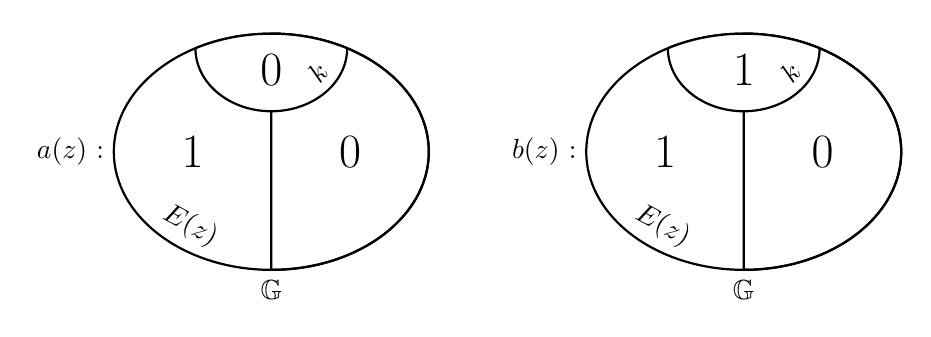
\begin{tikzpicture}
      \foreach \x/\lettre/\dansk in {0/a/0, 6/b/1} {
        \pgfmathparse{int(50+30*\dansk)}

        \node[left]       (\lettre) at (\x,0) {$\lettre(z)$ :};

        \draw[thick]      (\x,0) arc (180:540:2 and 1.5)
        node [pos=0.15, above, sloped] {$E(z)$}
        node [pos=0.25, below] {$\mathbb G$}
        coordinate [pos=0.83] (debutarc)
        coordinate [pos=0.67] (finarc)
        coordinate [pos=0.25] (fintrait);

        \draw [thick] (\x+4,0) arc (0:90:2 and 1.5) to (fintrait) arc (270:360:2 and 1.5);

        \draw[thick, fill=white] let \p1=(debutarc), \p2=(finarc) in
        (\p1) arc (180:360:{(\x2-\x1)/2} and 0.8cm)
        node [pos=0.5, above=2mm] {\LARGE{$\dansk$}}
        node [pos=0.8, above, sloped] {$k$}
        arc (180+360*0.67:180+360*0.83:2 and 1.5);

        \node at (\x+1,0) {\LARGE{1}};
        \node at (\x+3,0) {\LARGE{0}};
      }
    \end{tikzpicture}
  \end{center}

  Let $z<z'$.

  We want to show that $W(b(z))<W(a(z'))$.

  \begin{center}
    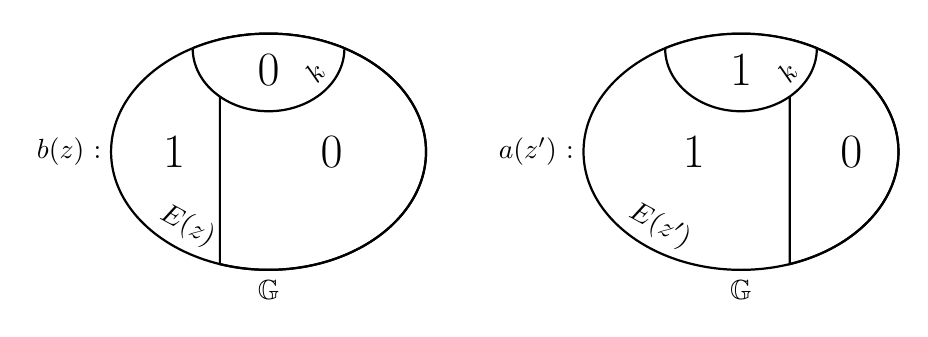
\begin{tikzpicture}
      \foreach \x/\lettre/\z/\dansk/\position in {0/b/z/0/0.2, 6/a/z'/1/0.3} {
        \pgfmathparse{int(50+30*\dansk)}

        \node[left] (\lettre) at (\x,0) {$\lettre(\z)$ :};

        \draw[thick]      (\x,0) arc (180:540:2 and 1.5)
        node [pos=0.15, above, sloped] {$E(\z)$}
        node [pos=0.25, below] {$\mathbb G$}
        coordinate [pos=0.83] (debutarc)
        coordinate [pos=0.67] (finarc)
        coordinate [pos=\position] (fintrait);

        \draw [thick] (\x+4,0) arc (0:{180-360*\position}:2 and 1.5) to (fintrait) arc ({180+360*\position}:360:2 and 1.5);

        \draw[thick, fill=white] let \p1=(debutarc), \p2=(finarc) in
        (\p1) arc (180:360:{(\x2-\x1)/2} and 0.8cm)
        node [pos=0.5, above=2mm] {\LARGE{$\dansk$}}
        node [pos=0.8, above, sloped] {$k$}
        arc (180+360*0.67:180+360*0.83:2 and 1.5);

        \node at ({\x+1.1-6*(0.25-\position)},0) {\LARGE{1}};
        \node at ({\x+3.1-6*(0.25-\position)},0) {\LARGE{0}};
      }
    \end{tikzpicture}
  \end{center}

  We are going to create two permutation $\sigma_1,\sigma_2\in\mu$ such as
  $\sigma_1 b(z)<_\kappa \sigma_2 a(z')$:

  \begin{center}
    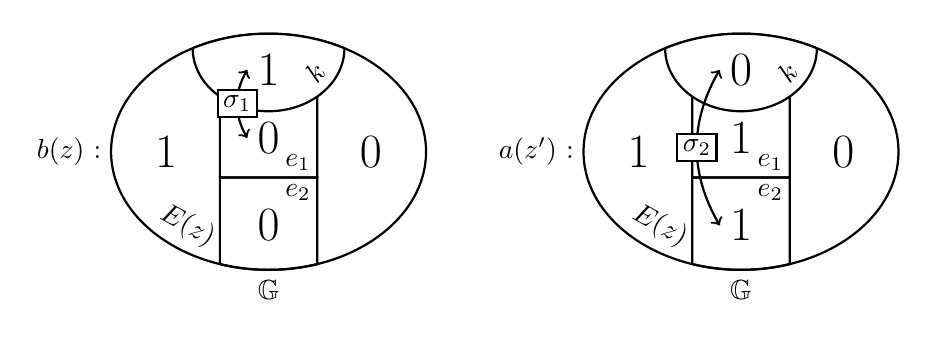
\begin{tikzpicture}
      \def\positionun{0.2}
      \def\positiondeux{0.3}
      \foreach \x/\lettre/\dansk/\aumilieu/\position in {0/b(z)/1/0/\positionun, 6/a(z')/0/1/\positiondeux} {
        \pgfmathparse{int(50+30*\dansk)}

        \node[left] (\lettre) at (\x,0) {$\lettre$ :};

        % Contour principal
        \draw[thick]      (\x,0) arc (180:540:2 and 1.5)
        node [pos=0.15, above, sloped] {$E(z)$}
        node [pos=0.25, below] {$\mathbb G$}
        coordinate [pos=0.83] (debutarc)
        coordinate [pos=0.67] (finarc)
        coordinate [pos=\positionun] (fintrait1)
        coordinate [pos=\positiondeux] (fintrait2);

        % Traits au centre
        \draw [thick]
        let \p1=(fintrait1), \p2=(fintrait2) in
        (fintrait1) arc ({180+360*\positionun}:{180+360*\positiondeux}:2 and 1.5)
        to ++ (0,1.1) coordinate (milieutrait2) node [below left, inner sep=2] {$e_2$} node [above left, inner sep=2] {$e_1$}
        to node [below=8] (e2\dansk) {\LARGE{\aumilieu}} node [above=5] (e1\dansk) {\LARGE{\aumilieu}} ++  ({\x1-\x2},0)
        to (fintrait1);
        \draw [thick]
        let \p1=(fintrait1), \p2=(fintrait2) in
        (milieutrait2) to + (0,1.1)
        arc ({360*\positionun}:{360*\positiondeux}:2 and 1.5)
        to ++ (0,-1.1)
        to cycle;

        % Zone pour k
        \draw[thick, fill=white]
        let \p1=(debutarc), \p2=(finarc) in
        (\p1) arc (180:360:{(\x2-\x1)/2} and 0.8cm)
        node [pos=0.5, above=2mm] (dansk\dansk) {\LARGE{$\dansk$}}
        node [pos=0.8, above, sloped] {$k$}
        arc (180+360*0.67:180+360*0.83:2 and 1.5);

        % 0 et 1 extrêmaux
        \node at (\x+0.7,0) {\LARGE{1}};
        \node at (\x+3.3,0) {\LARGE{0}};
      }

      % Flèches
      \draw [<->, thick] (e20.west) to [bend left] node [inner sep=2, fill=white, draw] {$\sigma_2$} (dansk0.west);
      \draw [<->, thick] (e11.west) to [bend left] node [inner sep=2, fill=white, draw] {$\sigma_1$} (dansk1.west);
    \end{tikzpicture}
  \end{center}

  Since there is some $r\in \D$ such that $z<r<z'$,
  \[\forall g\in \mathbb G\setminus k, \pi_2(g,r)\in]z,z'[,\]
  so $|\pi_2^{-1}(]z,z'[)|\geq|G\setminus k|$. And because $s$ is a bijection,
  \[|\pi_2^{-1}(]z,z'[)|=|s^{-1}(\pi_2^{-1}(]z,z'[))|= |f^{-1}(]z,z'[)|.\]

  Therefore $|E(z')\setminus E(z)|\geq|G\setminus k|\geq |k|$, then because
  $E(z')\setminus E(z)$ is infinite we can divide it in two sets $e_1$ and
  $e_2$ of same cardinality. Then there are two injections $\iota_i$ from $k$ to
  $e_i$. Define $\sigma_i$ as $\underset{g\in k}{\text{\LARGE $\circ$}}
  \tau(g,(\iota_i(g))$.

  \begin{center}
    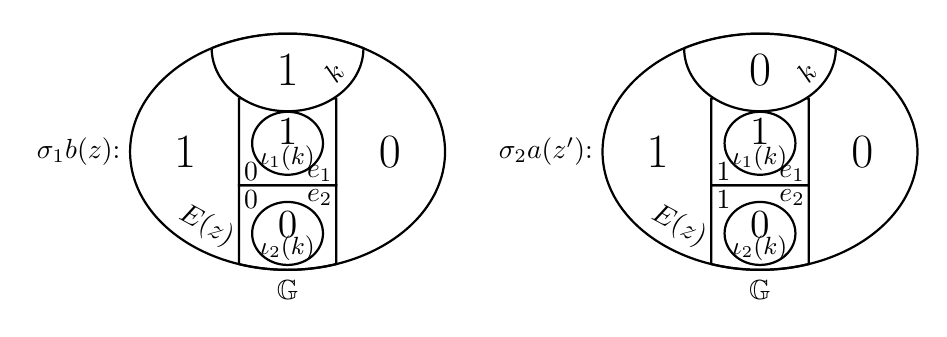
\begin{tikzpicture}
      \def\positionun{0.2}
      \def\positiondeux{0.3}
      \foreach \x/\lettre/\dansk/\aumilieu/\indice/\position in {0/b(z)/1/0/1/\positionun, 6/a(z')/0/1/2/\positiondeux} {
        \pgfmathparse{int(50+30*\dansk)}

        \node[left] (\lettre) at (\x,0) {$\sigma_\indice\lettre$:};

        % Contour principal
        \draw[thick]      (\x,0) arc (180:540:2 and 1.5)
        node [pos=0.15, above, sloped] {$E(z)$}
        node [pos=0.25, below] {$\mathbb G$}
        coordinate [pos=0.83] (debutarc)
        coordinate [pos=0.67] (finarc)
        coordinate [pos=\positionun] (fintrait1)
        coordinate [pos=\positiondeux] (fintrait2);

        % Traits au centre
        \draw [thick]
        let \p1=(fintrait1), \p2=(fintrait2) in
        (fintrait1) arc ({180+360*\positionun}:{180+360*\positiondeux}:2 and 1.5)
        to ++ (0,1) coordinate (milieutrait2) node [below left, inner sep=1] {$e_2$} node [above left, inner sep=1] {$e_1$}
        to node [below=6, inner sep=3] (e2\dansk) {\Large{0}} node [above=12.5, inner sep=2] (e1\dansk) {\Large{1}} ++  ({\x1-\x2},0) node [below right, inner sep=1.5] {\aumilieu} node [above right, inner sep=1.5] {\aumilieu}
        to (fintrait1);
        \draw [thick]
        let \p1=(fintrait1), \p2=(fintrait2) in
        (milieutrait2) to + (0,1.1)
        arc ({360*\positionun}:{360*\positiondeux}:2 and 1.5)
        to ++ (0,-1.1)
        to cycle;

        % Cercles
        \draw [thick] (e1\dansk.north) arc (90:450:0.45 and 0.4) node [above=0,pos=0.5, inner sep=1] {\small$\iota_1(k)$};
        \draw [thick] (e2\dansk.north) arc (90:450:0.45 and 0.4) node [above=0,pos=0.5, inner sep=1] {\small$\iota_2(k)$};

        % Zone pour k
        \draw[thick, fill=white]
        let \p1=(debutarc), \p2=(finarc) in
        (\p1) arc (180:360:{(\x2-\x1)/2} and 0.8cm)
        node [pos=0.5, above=2mm] (dansk\dansk) {\LARGE{$\dansk$}}
        node [pos=0.8, above, sloped] {$k$}
        arc (180+360*0.67:180+360*0.83:2 and 1.5);

        % 0 et 1 extrêmaux
        \node at (\x+0.7,0) {\LARGE{1}};
        \node at (\x+3.3,0) {\LARGE{0}};
      }
    \end{tikzpicture}
  \end{center}

  Let $g\in\mathbb G$.

  If $g\in k$ then
  \[(\sigma_1 b(z))_g=b(z)_{\underset{\notin E(z)\cup k}
  {\underbrace{\sigma_1^{-1}(g)}}}=0<1=(\sigma_2 a(z'))_g=
  a(z')_{\underset{\in e_2}{\underbrace{\sigma_2^{-1}(g)}}}.\]

  If $g\in \iota_1(k)$ then
  \[(\sigma_1 b(z))_g=b(z)_{\underset{\in k}{\underbrace{\sigma_1^{-1}(g)}}}=
  1=(\sigma_2 a(z'))_g=a(z')_{\underset{=g\in e_1}
  {\underbrace{\sigma_2^{-1}(g)}}}.\]

  If $g\in \iota_2(k)$ then
  \[(\sigma_1 b(z))_g=b(z)_{\underset{=g \notin E(z)\cup k}
  {\underbrace{\sigma_1^{-1}(g)}}}=0=(\sigma_2 a(z'))_g=a(z')_{\underset{\in k}
  {\underbrace{\sigma_2^{-1}(g)}}}.\]

  Else
  \[(\sigma_1 b(z))_g=a(z)_g\leq (\sigma_2 a(z'))_g=a(z')_g.\] \\

  Hence $\sigma_1b(z)<_\kappa \sigma_2a(z')$, so by $\kappa$-Pareto
  $W(\sigma_1b(z))<W(\sigma_2a(z'))$.

  Furthermore, since $\sigma_1,\sigma_2\in\mu$, by $\mu$-anonymity we have
  $W(\sigma_1b(z))=W(b(z))$ and $W(\sigma_2a(z'))=W(a(z'))$.

  So $W(b(z))<W(a(z'))$, so $[W(a(z)),W(b(z))]$ and $[W(a(z')),W(b(z'))]$
  are disjoint and not reduced to one element (since $a(z)<_\kappa b(z)$), so to each real
  we can associate a unique and disjoint interval which is not a singleton. That is absurd because
  we could then associate an element of $\mathbb D$ to each interval (by choosing one in the interval, by density),
  contradicting the strict inequality of the cardinals of $\mathbb S$ and $\mathbb D$.
\end{proof}



\bibliographystyle{alpha}
\bibliography{bibliography}
\end{document}
